\documentclass[a4paper,12pt]{report}
\newcommand{\scare}[1]{`#1'} 

\title{Broadcast Machine}
\author{Christian Bryan, Greg Opperman, Drew Wilson}

\usepackage{graphicx}
\usepackage{verbatim}
\usepackage{hyperref}

\begin{document}

% We need title page here. It has to be formatted as per the schools specs.
\begin{titlepage}
  \topmargin 0.5in
  \headheight 0in
\begin{center}
  \begin{flushright}
Project Number: MQP-CEW-0702\\
\end{flushright}
\vspace*{40mm}
Broadcast Machine\\
A Major Qualifying Project Report:\\
submitted to the Faculty\\
of the\\
WORCESTER POLYTECHNIC INSTITUTE\\
in partial fulfillment of the requirements for the\\
Degree of Bachelor of Science\\
By\\
\makebox[2in]{\hrulefill}\\
Christian Bryan\\
\vspace*{10mm}
\makebox[2in]{\hrulefill}\\
Greg Opperman\\
\vspace*{10mm}
\makebox[2in]{\hrulefill}\\
Drew Wilson\\
\vspace*{10mm}
\today\\
\vspace*{10mm}
\begin{flushleft}
  1. Internet\\
  2. video\\
  3. php\\
\end{flushleft}
\begin{flushright}
Approved:\\
\vspace*{10mm}
\makebox[2in]{\hrulefill}\\
Professor Craig E. Wills\\
\end{flushright}
\end{center}
\end{titlepage}

\chapter*{Abstract}
% TODO: One paragraph describing the project.
% FOR: CJ
% NOTE: It's gotta be 80 words or less.
With the prevalence of high-speed Internet and low-cost production equipment, Internet video publishing has rapidly come into the 
mainstream.
The original Broadcast Machine was an open-source application designed to allow Video producers to easily publish their work on the web, but was plagued with several problems.
Through careful evaluation and the use of popular software development techniques, we successfully rebuilt Broadcast Machine to be stable, scalable, maintainable and usable.

\tableofcontents

\chapter{Introduction}
% TODO: Describe the project goals and summarize the topics covered.
% FOR: CJ
With the prevalence of high-speed Internet and low-cost production equipment, Internet video publishing has rapidly come into the 
mainstream. Independent video publishers now have the ability to create professional videos and reach thousands of viewers with consumer-level equipment and little technical skill. There are several ways in which a video producer can publish videos online. Services like Youtube and Blip.tv offer free hosting for videos, and many content management systems offer plugins for publishers to distribute video files.

Created by the Participatory Culture Foundation, Broadcast Machine sought to fill the gap between centralized video hosting services and tacked-on content management system plugins by offering a complete video publishing solution for independent media producers. However, Broadcast Machine was plagued by several problems, and development was abandoned.

The main goal of this project was to take the ideas that had driven the development of the first version of Broadcast Machine and create a piece of software that was more usable and maintainable.
The original code base had been abandoned because the maintainers felt that it was taking up to much time and that any further work was unlikely to be fruitful.
The first part of this project was to identify the problems that the previous developers were running into and what their underlying causes were.
After in-depth interviews with the previous developers and an extensive review of the existing code,\footnote{For documentation on the previous Broadcast Machine, refer to Appendix A.} we identified problems with the previous Broadcast Machine and created a plan to prevent them in the next version.

\section{Topics}
This report details the methodologies and technologies that were used in the re-imagining of the Broadcast Machine package.
In Chapter 2 we will introduce the background of the package and its original maintainers as well as outline the deficiencies that were seen to impede the development of the original implementation.
In Chapter 3 there is a detailed discussion of the requirements necessary to prevent these problems from reoccurring, with each requirement analyzed and discussed in detail.
In Chapter 4 we discuss the implementation details that result from these requirements.
Following the chapters on design and implementation, in Chapter 5, we show the system in action with a full walkthrough of the new software and a description of the functionality it provides.
Finally, in Chapter 6, our group discusses the results of the project, as well as features that our group was unable to implement and which ones we feel are necessary to the long-term success of the project. The future of the project is covered in Chapter 7. Finally, in Chapter 8, we close with a short reflection on the project.

\chapter{Background}

\section{Introduction}
% TODO: A good overview of the topics covered in the Background chapter. 
% FOR: CJ
In this section we take a look at the history of Broadcast Machine.
Our goal is to provide the reader with a framework to understand the reasons for this software's existence and the environment in which it is being built.
The importance of this software to the Participatory Culture Foundation should be noted.
As this foundation tries to promote freedom for content producers, the majority of its competitors are attempting the opposite.
Unfortunately this software has not thrived.
Due to decisions made early in the software's development and an lack of funds for its re-development Broadcast Machine has fallen by the wayside.
Our group has come to see Broadcast Machine as important player in the arena of Internet video and is dedicated to ensuring that it 
becomes viable again.

\section{Open-Source Software}
Open source software is an important part of the movement to democratize the media and Internet. 
This common goal is what ties together PCF's mission with that of the Free Software Movement. 
The goal of the Free Software Movement is to create software to increase the freedom of the public in general.\footnote{Richard Stallman, Why Software Should Be Free \url{http://www.gnu.org/philosophy/shouldbefree.html}}
Open-Source Software accomplishes this through its transparency, which inspires community development of software, and gives users the freedom to modify the software to suit their needs.
The software is free in the sense that there are no conditions in distributing or using it, except that users respect the freedom of the software.

Without free software, the Internet could not exist as a democratic medium.
Proprietary (meaning closed-source) software limits what users can or can't do with it, and does not give users the ability to modify code.
With proprietary software, users cannot \scare{own} software, even if they purchase it.
Instead, users pay for the privilege of using it.
Under this model, the software is less accessible and less usable (as users cannot fix problems on their own, and must rely on proprietary developer support).
On top of this, other developers cannot learn from existing code, or base new work on it without paying costly licensing fees.\footnote{Ibid} 


Open-source software aims to build a cultural community of developers who can use each other as resources, learning from existing code, and freely building upon it to create new technologies altogether.
This culture encourages technological progress in ways that competitive, closed-source software does not. 

\section{The Current State of Internet Video}
As bandwidth and storage become increasingly cheaper, the prevalence of video on the Internet has sharply risen over the past few years. 
In August 2006 alone, the number of people in the U.S who streamed video 
via the Internet totaled over 110 million people, which is comparable 
with the number of households that watch traditional television.\footnote{\url{http://paul.kedrosky.com/archives/2006/10/19/fun\_with\_intern.html}}
The Internet has allowed independent video producers a variety of platforms by which to publish and share their work. These platforms come 
in one of two forms: video hosting services, which offer a centralized location from which users can upload and share videos, and Content Management Systems (CMS), where users host and maintain their own collections of videos.

\subsection{Video Hosting Services}
Video hosting services are sites that offer free hosting and sharing of video files that users upload.
These sites, such as YouTube (\url{http://youtube.com}), Blip.tv (\url{http://blip.tv}), and Myspace Videos (\url{http://vids.myspace.com}) also offer social networking features, such as the ability to rate and comment on videos, as well as subscribe to videos posted by friends.
The largest and most popular video hosting service is Youtube, which garners 42.94\% of all traffic to online video sites.\footnote{\url{http://www.hitwise.com/press-center/hitwiseHS2004/videosearch.php}}. 

Video hosting services offer a convenient solution for video publishers 
to share videos with little technical expertise or resources, since bandwidth and hosting costs are shouldered by the service. These sites also allow users to embed videos into their own sites, giving them creative control over how the video is displayed. However, there are several limitations to this approach. In order to keep costs down and ensure that services remain possible under heavy traffic, most video hosting sites impose limitations that affect the quality of uploaded content. Having to service over 50,000 uploads a day, YouTube transcodes all of its videos to a lower resolution, and imposes a limitation on the length of video clips \footnote{\url{http://www.youtube.com/t/fact\_sheet}}. 

None of the major video hosting services allow adult or objectionable content.
Many sites regularly censor videos they deems inappropriate, including YouTube, who retains the right to control any and all content on its servers.
Often, videos aimed at displaying legitimate discourse or expression are lost to this censorship\footnote{\url{http://www.nytimes.com/2006/10/09/technology/09link.html?ex=1318046400&en=e311caef3c3cf222&ei=5090&partner=rssuserland&emc=RSS}}.
For many publishers, the only way to ensure that their videos are presented correctly is to host them independently, using a content management system.

\subsection{Content Management Systems}

A Content Management System, or CMS, is a blanket term referring to the wide array of pre-packaged software used to manage website content. CMSes can encompass software to create wikis, forums, and several other collaborative mediums. In general, CMSes provide a simple user interface for adding, editing, and removing content, while obfuscating technical details. Using a CMS, it would be possible to build and manage an entire site without having knowledge of the underlying technologies and code. Most CMSes also offer robust theming engines, allowing users confortable with HTML and CSS to easily customize the look and feel of their site. Currently, the two most popular CMSes are Drupal and Wordpress.

\subsubsection{Drupal}
Drupal allows users to easily set up, create, and moderate blogs, forums, webpages, newsletters, and picture galleries\footnote{\url{http://drupal.org/about}}.
Written in PHP, it requires either MySQL v3.23.17 or PostgreSQL 7.2 or above\footnote{\url{http://drupal.org/requirements}}.
Thousands of popular sites use Drupal\footnote{\url{http://drupalsites.com}}, including The Onion\footnote{\url{http://theonion.com}} and MTV's UK site\footnote{\url{http://mtv.co.uk/}}.

\subsection{Wordpress}
Wordpress one of the most popular weblogging applications, or a CMS designed specifically for posting text and image content by a small group of users.
Wordpress is built with PHP 4.2 and uses MySQL 3.23 as its database back-end. 
It was created with the vision of creating a powerful GPL-licensed Internet publishing platform based on open standards. 
The first version was released in 2001. 
Wordpress is blogging software designed to be installed on an individual's web host, either their own computer connected to a broadband connection or a commercial web host like Dreamhost or 1and1. Wordpress also offers hosted installations of its own software on their website.\footnote{\url{http://wordpress.org}}

Wordpress and Drupal both offer plugins for video publishing. However, there are currently no CMSes that directly address the needs of online video producers. There is a clear need for an easy to use, open-source, alternative to centralized video hosting service or complicated CMS plugins. With this in mind, the Participatory Culture Foundation (PCF), a Worcester-based non-profit, created Broadcast machine, an open-source video publishing platform.

\subsection {Broadcast Machine}
Broadcast Machine is a content management system for video publishing designed to deliver videos via several different methods. Primarily, 
it acted as video blogging software, where users could organize videos into channels. Users could also subscribe to these channels using any RSS reader or desktop video software, such as Miro (\url{http://getmiro.com}). Broadcast Machine targeted users with little technological experience to offer a simple, easy-to-use user experience, and promoted alongside Miro (formerly Democracy Player) as part of a multi-tiered Internet video platform, Broadcast Machine developed a strong following of users\footnote{A Google search of the phrase \textit{Powered by Broadcast Machine} returns approximately 6,700 results.}

Despite its popularity, Broadcast Machine was plagued by a number of problems due to poor architectural decisions and sloppy programming practices\footnote{PCF's bug tracker reports 67 serious, unfixed bugs as of the time of this writing.}. The original Broadcast Machine stored data in one of two ways: a MySQL database or a flat-file. However, model-layer logic was poorly abstracted from the rest of the application, and small differences between the two data-layer implementations caused several irreconcilable bugs. Since the program relied on a complicated and difficult to understand architecture, tracking down and fixing these problems became nearly impossible. Poor documentation, especially concerning Broadcast Machine's complex data structures made it especially difficult for others developers to work on the project. Due to the aforementioned issues and lack of funding, development of Broadcast Machine was abandoned in 2006, to the dismay of its dedicated users.

\section{Summary}
In this chapter we discussed the relavance of open source and free software. It is essential for the movement to democratize
media to include open source software. We also gave an overview of the current state of Internet video. There was a description of some
of the most common web hosting services and a number of content management systems that somewhat address the needs of video content
producers. As we have shown it is neccesary for us to design a system that better addresses the specific needs of video content producers.

\chapter{Design}

\section{Introduction}
Many of Broadcast Machine's current problems stem from its poor architectural implementation. 
To prevent these problems from happening in the future, the new Broadcast Machine must have a carefully-planned architecture that meets several design requirements.

\section{Ease of Use}
The most important requirement for Broadcast Machine is that it be easy to use. 
Broadcast Machine's target user, people who produce videos, should not need extensive technical knowledge in order to deploy and use the program. 
Just as a developer has almost no knowledge of how to shoot or edit a video, we should not expect the user to have any knowledge of PHP, RSS, or any of the technologies employed. 
Without being privy to any of the inner workings of the program, the user must be able to easily and intuitively publish videos and video channels via a simple administrative interface. 
Without any information besides their web server log in and password, the user should be able to set up Broadcast Machine by dropping the application into a folder accessible by a web server. 
The program should auto-configure itself on the first-run with a few simple clicks, even if the user is completely unaware of how his or her web server is set up. 
The application must detect server configurations that may interfere with its behavior, and handle those special cases gracefully. 
Likewise, viewers with any level of computer proficiency must be able to easily browse and download videos, and subscribe to their favorite channels.

In order to ensure the best user experience possible, the new Broadcast Machine must be stable. In addition, it should preserve all of the functionality of its previous incarnation, while containing none of the unpredictable behavior.

\subsection{Customizable} 
A major feature of both the former Broadcast Machine and many other CMSes is the ability to customize the look and feel of an installation that fits the user's own personal style. 
As before, the application must be designed with a robust theming engine so that a user with only basic HTML and CSS knowledge can easily customize the website to suit his or her needs. 
Each users' site layout, or theme, will have the potential to look drastically different from each other with only minimal modifications to CSS and template code. 
The templates must be abstracted from the functional code, so that users need not worry about breaking the logic of the application or having to dig deep into obscure files to modify the layout. 
Users should also have the ability to easily switch between layouts. 


\subsection{Extensible} 
Similarly, the application logic of Broadcast Machine must be structured so that it may be easily modified and maintained by any developer with relevant skills. 
The layout of the application should appear logical and concise, with a modular architecture to encourage programmers to freely add onto Broadcast Machine's feature set in order to meet their requirements.
The architecture should be transparent and have a well-documented API so that theses developers can start extending Broadcast Machine without exhaustive knowledge of the program, but merely a solid grasp of the documented data structures and class layouts. 
When features need to be added, the developers should be able to do so while maintaining the same architectural pattern and preserving the structure of the application, by adding only a few functions or classes. 
A well-structured, extensible architecture will prevent poor programming practices by encouraging developers to replicate the design patterns used to create the foundation of the application.


\subsection{Flexible}
Broadcast Machine must be flexible enough so that it can be re-factored easily. 
Functionality should be abstracted and delegated so that major changes to one part of the code will not affect another. 
For example, we may decide later that we would like to use a different type of database. 
We should be able to swap out the back end without having to modify the entire application, and without significantly affecting the user experience. 
In the event that bugs occur, localizing them to a specific section of code and implementing a fix should be possible without the fix appearing to be makeshift. 
Developers should not need to dig through a large amount of application code before finding the section that they need to edit. 


\subsection{Compatible}
The new Broadcast Machine must work across several different platforms. 
While impossible to guarantee compatibility with all web server configurations, Broadcast Machine most work on the most common web server setups. 
This includes any Apache web server with a minimal amount of installed modules, and most major hosting services (Dreamhost, 1And1, etc). 

\section{Summary}
In this chapter we discussed the target audience for the software and the design requirements of the system. The target audience for 
Broadcast Machine is primarily non-technical users who have experience with 
video editting, but who are not 
necessarily familiar with web-programming or web-design. As such the program needs to be designed with those people in mind.
Many other content management systems fail in this regard. Despite the need for a simple interface, the system needs to be 
customizable. For this reason a robust theming engine is neccesary. Since the each install of Broadcast Machine is seperate and the system 
is not central maintained, it is also important 
to have a consistent code structure that allows for third party developers and more technical users to write extensions. 
Flexibility and compatibility are two additional requirements of the system. The software must be able to 
have components removed or 
replaced without compromising the entire code base. Finally, the system needs to be designed with the most common web host platforms in 
mind. It is essential that Broadcast Machine be compatible with the leading commercial web hosts.

\chapter{Implementation}

\section{Introduction}
Based on the design requirements it is clear that we need an architecture for abstracting the code into multiple layers. In this chapter 
we discuss how we implemented the system. We explain the Model-View-Controller architecture and how we applied it to 
Broadcast Machine. We discuss the programming language chosen and the expected hosting environment. This chapter goes into detail about 
the various controllers, the database model, and the views of the system. This chapter deals with the specifics of the code and 
implementation. 

\section{Model-View-Controller}
It became clear that the program architecture needed to be modularized into three separate parts. First, the presentation layer needed to 
be separated from program logic in order to create a theming system by which users with basic HTML and CSS knowledge could customize the style of their site. In order to make the program both extensible and flexible for developers looking to add onto or modify existing Broadcast Machine code, it became necessary to further abstract data storage to be independent of both the presentation layer and the rest of the program architecture. This separates the program into three layers, following the Model-View-Controller design pattern, or MVC\footnote{\url{http://www.martinfowler.com/eaaDev/uiArchs.html}}, as shown in Figure 4.1.


\begin{figure}[htp]
\begin{center}
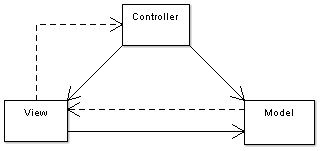
\includegraphics[scale=0.6]{./images/mvc.png}
\end{center}
\caption{Interaction between layers in MVC}
\end{figure}
In a pure Model-View-Controller architecture, all data is represented by the Model layer. The layer that the user interacts with, namely user-interface of the application, is represented in the View layer. The Controller layer represents the logic of the application, and in most cases, handles interactions between the Model and View layers. These interactions are shown in Figure 4.1, with solid lines representing direct interactions, and dotted lines representing indirect interactions. Although in the general definition of this design pattern, the view can take user input and push it directly to the model, in most implementations it passes input to the controller for processing (input-validation), which in turn pushes the input to the model. Likewise, the view can also request data from the controller, who queries the Model layer. The query is then passed to the View for display and further user interaction.

\section{Languages and Tools}
There are several frameworks for implementing Model-View-Controller web applications, currently the most popular of which is Ruby on Rails. Ruby on Rails provides advanced features that allow automatic, rapid-prototyping of MVC applications, and object-relational mapping for controller interaction with the model layer, meaning that all data is automatically assigned to a class object based its structure.\footnote{\url{http://rubyonrails.org}} However, as a relatively new language, Ruby on Rails has not been as widely adopted as other, more established languages. Few basic web hosting plans support Ruby on Rails. 

To satisfy the requirement that Broadcast Machine be compatible with as many hosting and web server configurations as possible, we chose to write the application in PHP\footnote{\url{http://php.net}} running under Apache web servers\footnote{\url{http://apache.org}}. PHP is currently one of the most popular web scripting languages, while Apache is also the most prevalent web server amongst low-cost web hosts and developers running personal web servers.\footnote{\url{http://news.netcraft.com/archives/2007/01/05/january\_2007\_web\_server\_survey.html}}
Another advantage is that it is common for PHP and Apache to be installed alongside one another. Apache's support for per-directory configurations via an .htaccess file make it easy for users and developers to customize the environment without specialized administrator access; PHP offers object-oriented programming features that allow for the development of a MVC application that adopts many of the design principles and features of a Rails framework.

Similarly, MySQL is an open-source Database Management System (DBMS) that is one of the most widely-used Structured Query Language (SQL) implementations for data storage, alongside enterprise-level applications such as Oracle. Like PHP, MySQL comes installed by default with most hosting plans, and many hosts offer user-friendly interfaces to set up and manage databases. After a database has been created by the user with one of these tools, deploying the data layer of the application would be automated by a script. In terms of scalability, MySQL's performance rivals that of many enterprise-level DBMSes, especially when executing simple queries to create, read, update and delete small amounts of data. PHP offers several functions to interact with MySQL, making it the ideal choice for the data layer of the application.

\section{Application layout}
Using the aforementioned languages and tools, the traditional Model-View-Controller pattern was modified slightly for Broadcast Machine, in order for each layer to logically handle requests and delegate responsibilities as best as possible, as shown in Figure 4.2.

\begin{figure}[htp]
\begin{center}
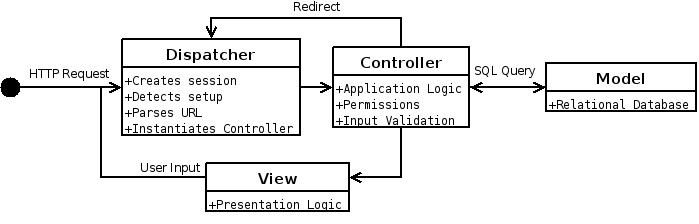
\includegraphics[scale=0.5]{./images/flow.png}
\end{center}
\caption{Interaction Between Application Layers}
\end{figure}

First, Broadcast Machine receives an incoming HTTP request and invokes the dispatcher. The dispatcher is a kind of meta-controller for Broadcast Machine, that takes in a URL request and any POST data from the user, and does any work necessary before the requested controller is instantiated. The dispatcher first checks to make sure that Broadcast Machine's .htaccess file, configuration file, and database are properly set up before invoking the proper controller. If Broadcast Machine is found to be not set up, then the dispatcher automatically ignores the URL request and invokes the setup controller to initiate the proper step of the set up process. If the application is set up, then the dispatcher parses the URL request and invokes the appropriate controller. The dispatcher expects URLs in the following format:

\textbf{http://baseurl/[controller]/[param]/../[param]/} \\

If no controller is given, the dispatcher by default invokes the Channel Controller. Beyond the type of controller requested, the dispatcher delegates the responsibility of interpreting URL parameters to the invoked controller.

\section{Controllers}

All of the application logic for Broadcast Machine resides in the controller layer. Controllers are classes of objects that perform a set of related tasks. 

\subsection*{View Controllers}
View Controllers are the most common type of controller in Broadcast Machine, and are responsible for handling all of the requests that result in template rendering. All view controllers inherit some functionality and requirements from the ViewController Abstract Class. The ViewController aggregates (contains) the DatabaseController, whose specific implementation is defined by a configuration variable and automatically instantiated.\footnote{By default, Broadcast Machine uses the MySQLController.} In a similar fashion, the ViewController automatically aggregates an instance of Smarty, the default templating engine of choice.\footnote{For more information on Smarty, see the \textbf{View} section below.} ViewControllers also inherit the ability to determine permissions and assign alerts from their abstract parent. The ViewController also provides a uniform interface for invoking a template.

\begin{figure}[htp]
\begin{center}
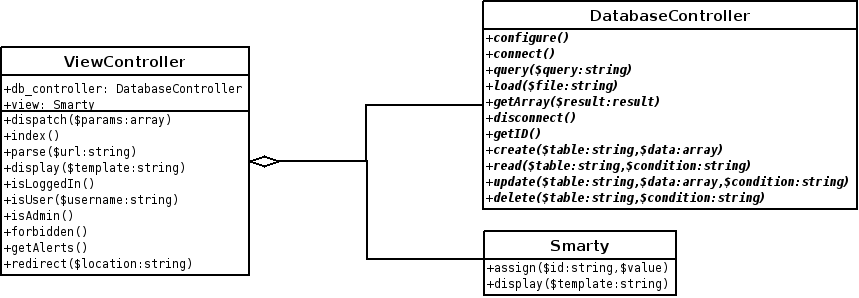
\includegraphics[scale=0.5]{./images/controllers.png}
\end{center}
\caption{ViewController API}
\end{figure}

As shown by Figure 4.3, the ViewControllers are responsible for taking in an array of URL parameters\footnote{Recall that URLs are parsed by the dispatcher into an array before instantiating a ViewController}, and invoking the correct method and parameters. For example, if the ChannelController is called with the following parameters: \\

\textbf{[0] = channel, [1] = cowboys, [2] = edit} \\

The Channel Controller, in the dispatch() method, assumes that \scare{cowboys} is the name of the channel, and invokes the edit method with \scare{cowboys} as the target channel. There are five classes that implement the ViewController interface: the Setup, Channel, Video, Tag, and User Controllers. \\

\subsubsection{SetupController}
The \textbf{SetupController} is responsible for completing a Broadcast Machine installation, as well managing site  and database settings after BM has been set up. The SetupController has the following methods (corresponding URL parameters in parentheses):
\begin{description}
\item{\textbf{index (/setup/): }calls settings() by default when there are no parameters, if a user is logged in and has admin privileges.}
\item{\textbf{write\_htaccess (/setup/cleanurls/): }The first step of setup, sets up the .htaccess file for proper URL handling.}
\item{\textbf{settings (/setup/settings): } Allows an admin to set up or modify site and database settings.}
\item{\textbf{write\_bm2conf: } Writes BM's configuration file.}
\item{\textbf{firstuser (/setup/firsuser): } Allows user to create the first admin log-in.} \\
\end{description} 

\subsubsection{ChannelController}
The \textbf{ChannelController} is responsible for aggregating and managing data related to channels, or collections of videos. The ChannelController has the following methods:
\begin{description}
\item{\textbf{index (/channel/): } Calls all() by default when there are no parameters.}
\item{\textbf{all (/channel/all): } Displays all channels, as well as a short list of videos in those channels and associated tags.}
\item{\textbf{add (/channel/add): } Adds a channel to the database.}
\item{\textbf{edit (/channel/channelname/edit): } Modifies channel \textit{channelname}.}
\item{\textbf{show (/channel/channelname/): } Shows details for a channel.}
\item{\textbf{RSS (/channel/channelname/RSS): } Displays a channel's RSS feed.}
\item{\textbf{remove (/channel/channelname/remove): } Deletes a given channel from the database.} \\
\end{description} 

\subsubsection{VideoController}
The \textbf{VideoController} is responsible for aggregating and managing data related to videos. The VideoController has the following methods:
\begin{description}
\item{\textbf{index (/video/): } calls all() by default when there are no parameters.}
\item{\textbf{all (/video/all): } Displays all videos, as well as associated tags.}
\item{\textbf{add (/video/add): } Adds a video to the database.}
\item{\textbf{edit (/video/videoname/edit): } Modifies video \textit{videoname}.}
\item{\textbf{show (/video/videoname/): } Shows details for a video.}
\item{\textbf{download (/video/videoname/download): } Increments a video's download count and serves up the video file.}
\item{\textbf{remove (/channel/videoname/remove): } Deletes a given video from the database.} \\
\end{description} 

\subsubsection{TagController}
The \textbf{TagController} is responsible for aggregating and managing data related to tags, or categories for videos and channels. The TagController has the following methods:
\begin{description}
\item{\textbf{index (/tag/): } calls all() by default when there are no parameters.}
\item{\textbf{all (/tag/all/): } Displays all tags for channels and videos.}
\item{\textbf{show (/tag/tagname/): } Shows all videos and channels tagged with \textit{tagname}.}
\item{\textbf{RSS (/tag/RSS/): } Displays an RSS feed for videos tagged with \textit{tagname}.} \\
\end{description} 

\subsubsection{UserController}
The \textbf{UserController} is responsible for aggregating and managing data related to users. The UserController has the following methods:
\begin{description}
\item{\textbf{index (/user/): } calls show() for current user by default when there are no parameters, or presents a login screen if there is no active session.}
\item{\textbf{signup (/user/signup/): } Registers a user.}
\item{\textbf{login (/user/login/): } Begins a session with proper user credentials.}
\item{\textbf{all (/user/all/): } Shows all users (admin-only).}
\item{\textbf{show (/user/username/show): } Shows information for user \textit{username}.}
\item{\textbf{edit (/user/username/edit/): } Allows a user to edit their own information.}
\item{\textbf{remove (/user/username/remove/): } Allows a user or admin to remove an account.} \\
\end{description}

\subsection*{Database Controllers}
Database Controllers are controller classes that manage queries to the model layer. In implementing MySQL database support for Broadcast Machine, several abstraction layers were created to make it easy to add new DBMS support to the application.
\begin{figure}[htp]
\begin{center}
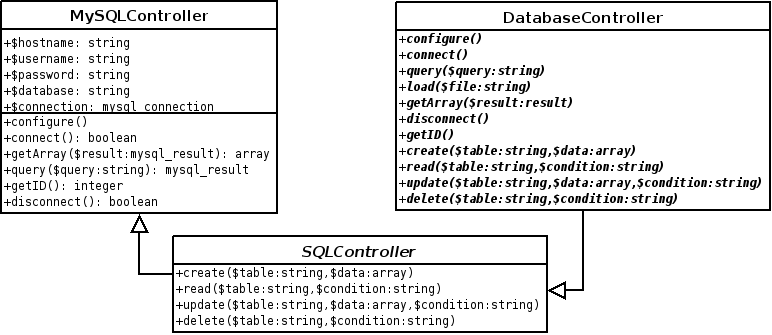
\includegraphics[scale=0.5]{./images/mysql.png}
\end{center}
\caption{MySQLController Inheritance Diagram}
\end{figure}

As you can see in Figure 4.4, the abstract class \textbf{DatabaseController} defines the API by which all database controllers are expected to behave, witch functions to configure, connect, and disconnect from database sessions, as well as to create, read, update, and delete data, as well as to parse record sets into arrays and retrieve the unique ID of the last inserted record.

The \textbf{SQLController} extends the Database controller by providing the create, read, update, and delete functions to build and execute SQL queries for all of these functions. This abstraction provides these functions for any developer writing controllers for any other SQL implementation (such as SQLite or PostgreSQL) automatically, so long as their implementation extends the SQLController class.

Finally, the MySQL controller is a concrete implementation of the DBMS used in Broadcast Machine. It implements functions to maintain database connections by calling MySQL-specific functions in PHP, allowing other Broadcast Machine controllers to interact with the model layer.

\section{Model}
Data for Broadcast Machine can be broken down into five main entities: Channels, Videos, Tags, Users, and Settings. This is shown in Figure 4.5. Settings, a group of data with no relation to the other entities, are stored in the file bm2\_conf.php, while the rest of the data is stored as a relational MySQL database (see Languages and Tools above). The entities and their relationships are shown below.
\begin{figure}[htp]
\begin{center}
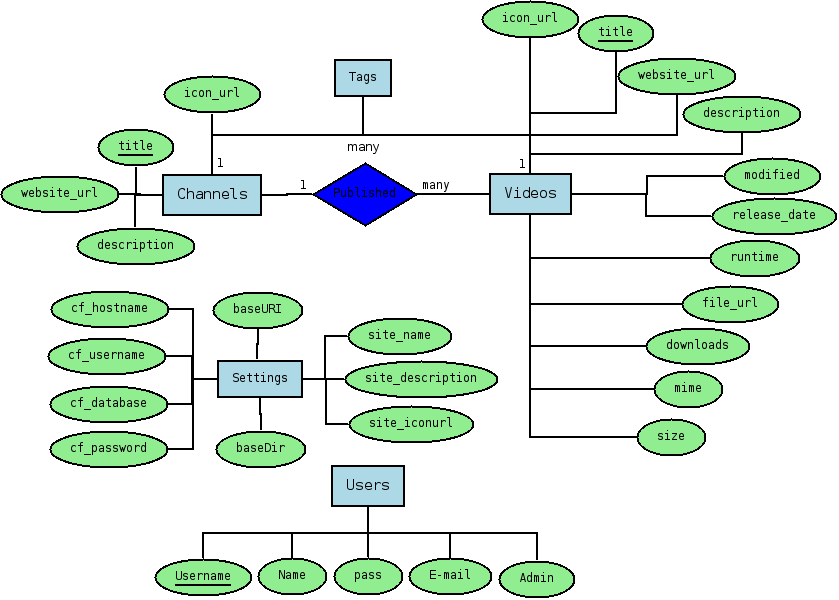
\includegraphics[scale=0.45]{./images/er.png}
\end{center}
\caption{Entity-Relationship Diagram}
\end{figure}

\subsection*{Channels}
Channels used to organize videos into collections. Users can either view channels through Brodcast Machine, or subscribe to Channels via RSS or Miro. Each channel has the following attributes:
\begin{description}
\item{\textbf{title: } The name of the channel. Must be unique.}
\item{\textbf{description: } A short summary of what the channel contains.}
\item{\textbf{website\_url: } An optional link to the channel homepage.}
\item{\textbf{icon\_url: } The address of a channel icon, or logo.} \\
\end{description}
Each channel can have several videos published to it, meaning those videos will appear as part of the channel. Channels can also be tagged with descriptive keywords (see Tags).

\subsection*{Videos}
\begin{description}
\item{\textbf{title: } The name of the video. Must be unique.}
\item{\textbf{description: } A short summary of what the video is about.}
\item{\textbf{website\_url: } An optional link to the video publisher homepage.}
\item{\textbf{modified: } A timestamp of the last time a video was updated.}
\item{\textbf{release\_date: } When the video was uploaded to Broadcast Machine.}
\item{\textbf{runtime: } The length of the video, in seconds.}
\item{\textbf{file\_url: } The location of the video file.}
\item{\textbf{downloads: } The number of times the video has been downloaded.}
\item{\textbf{mime: } MIME-type of the video.\footnote{MIME is an international standard that defines what kind of content a file contains.}}
\item{\textbf{size: } Size of the video.} \\
\end{description}

\subsection*{Tags}
Tags, or categorical words that describe another entity, are represented by two database tables, channel\_tags and video\_tags. Each tag contains the unique ID of the channel or video it refers to, as well as the one-word tag itself. Tags allow channels and videos to be aggregated and organized by category or theme, allowing videos and channels to belong to several categories at once.

\subsection*{Users}
Users are members of a Broadcast Machine site, and fall into one of two categories. Administrators, or admins, are users who manage the site and are responsible for adding, updating, and removing content. It's possible for site admins to restrict all or some videos on their site to be viewable only by registered members. Information needed to represent users is as follows:

\begin{description}
\item{\textbf{username: } The nickname that a user logs in as.}
\item{\textbf{name: } User's real-life name.}
\item{\textbf{pass: } A hash of the user's password.}
\item{\textbf{email: } User's e-mail address.}
\item{\textbf{admin: } Whether or not the user has administrative privileges.} \\
\end{description}

\subsection*{Settings}

Site settings pertain to global information about the specific Broadcast Machine installation. They typically include information needed by the dispatcher before connecting to the database or instantiating a controller. Site settings include:

\begin{description}
\item{\textbf{baseURI: } The URI of the root location of the BM installation. Used to dynamically generate links.}
\item{\textbf{baseDir: } The base directory of the BM installation. Used to properly include classes and files.}
\item{\textbf{site\_name: } The name of the site.}
\item{\textbf{site\_description: } A brief summary of the site.}
\item{\textbf{site\_iconurl: } A link to the logo of the site.} \\
\end{description}

Database connection settings are specific to the Database Management System being utilized. As such, each Database Controller is responsible for knowing which variables are set in the settings file and including them. By convention, all database settings are prefixed with \scare{cf} and are in the form \$cf\_varname. An example of typical database settings (in this case for the MySQLController): \\

\begin{description}
\item{\textbf{cf\_hostname: } The URI through which the database can be reached.}
\item{\textbf{cf\_database: } The name of the database.}
\item{\textbf{cf\_username: } Username needed to access database.}
\item{\textbf{cf\_password: } Password needed to access database.} \\
\end{description}

All settings, both for the Site and Database, are stored in bm2\_conf.php in Broadcast Machine's base directory.

\section{View}
The implementation of the presentation layer in Broadcast Machine is handled by Smarty, an open-source PHP templating engine. 
Smarty was chosen because it provides users with an easy way to create dynamic webpages without requiring that template developers deal directly with application logic or PHP, while still allowing users to customize each dynamically-generated views. In Smarty, data is assigned to templates via variables, much like in PHP. The View Controller assigns these variables before calling a template to be rendered, and Smarty automatically inserts the variables when rendering the template, fully removing the data presented from SQL or Controller logic.
Smarty also allows for simple flow control and special variable modifiers.
These variable modifiers allow the presentation layer to retain some control over how the data is filled, while keeping a suitable amount of abstraction.
For example, they can be used to capitalize strings, alternate colors of rows, or escape special characters.
Smarty then takes in the templates for the presentation layer and compiles them into PHP. The Smarty templates together and the View Controller are the components of the the user interface.

\section{Summary}
In this chapter we outlined the implementation of the software, as it followed from the design decisions. We used the 
Model-View-Controller architecture for the system because it provided us with a consistent framework. The framework also allowed us to 
abstract the different layers of the software in a way that was consistent with the design goals. Although there were a number of 
languages and tools available for creating our software, we decided on PHP because it was the most compatible with popular web hosts. This 
section also included detailed descriptions of the controllers (tag controller, the user controller, etc), their associated functions and 
their associated views. In the next chapter we will walk through the system and show it in action, from a user's perspective. 

\chapter{System in Action}

\section{Introduction}
This section details how installation and use of Broadcast Machine works, with a pictorial walkthrough of the various views and pages of Broadcast Machine. 
Through these concise illustrations of the software we hope to convey the full range of Broadcast Machine's features.

\section{Setup}
In this section we are going to take a look at how Broadcast Machine is initially set up on a user's server.
The initial step is downloading the archive that contains the software.
In the future, the software will be available through the project's home page.\footnote{\url{http://code.google.com/p/broadcastmachine}}
After the user downloads the file, they upload it to their server and unpack it into some directory that will be accessed by a web server.

\subsection{Clean URLs}
  \begin{figure}[htp]
  \begin{center}
  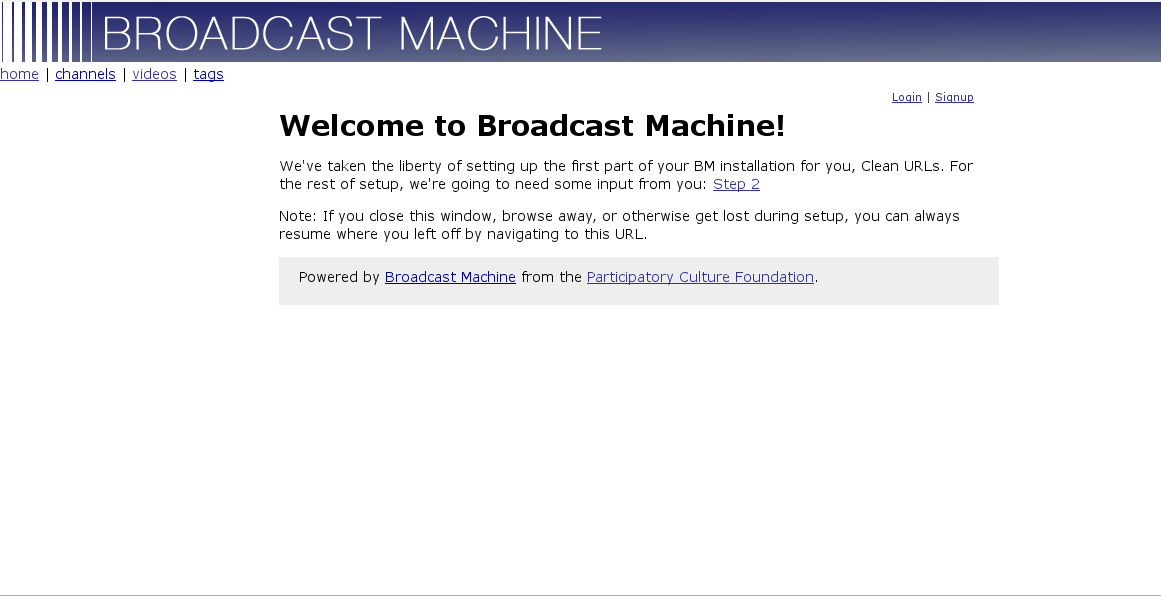
\includegraphics[width=150mm]{./images/setup1.png}
  \caption{Broadcast Machine Greeting Page}
  \end{center}
  \end{figure}
Figure 5.1 shows the first screen that a user encounters when installing Broadcast Machine displays a simple greeting.
In the background, the application is detecting the current server settings and is attempting to set up Apache's .htacces file, which allows for clean, user-friendly URLs using mod\_rewrite.
A few settings such as the permissions on directories and the type of PHP modules installed are also detected.

\subsection{Settings}
\begin{figure}[htp]
\begin{center}
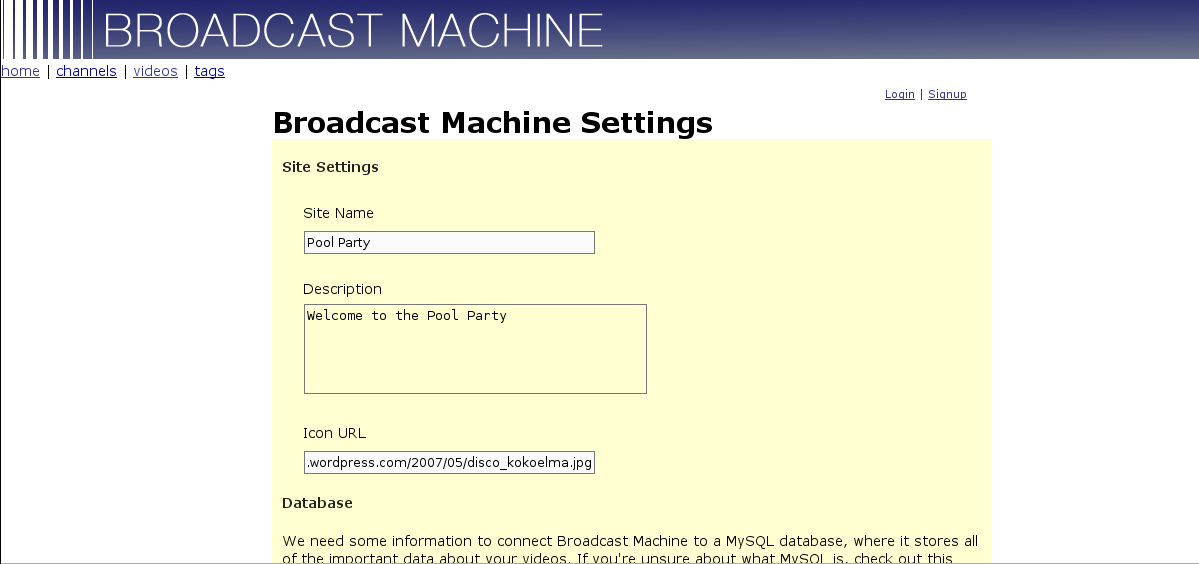
\includegraphics[width=150mm]{./images/setup2.png}
\caption{Site Settings Page}
\end{center}
\end{figure}

Figure 5.2 shows the second setup step, where the basic information about the installation is entered.
We collect information such as the title and description of the site, as well as all of the information we need to connect to the database.

\subsection{First User}
\begin{figure}[htp]
\begin{center}
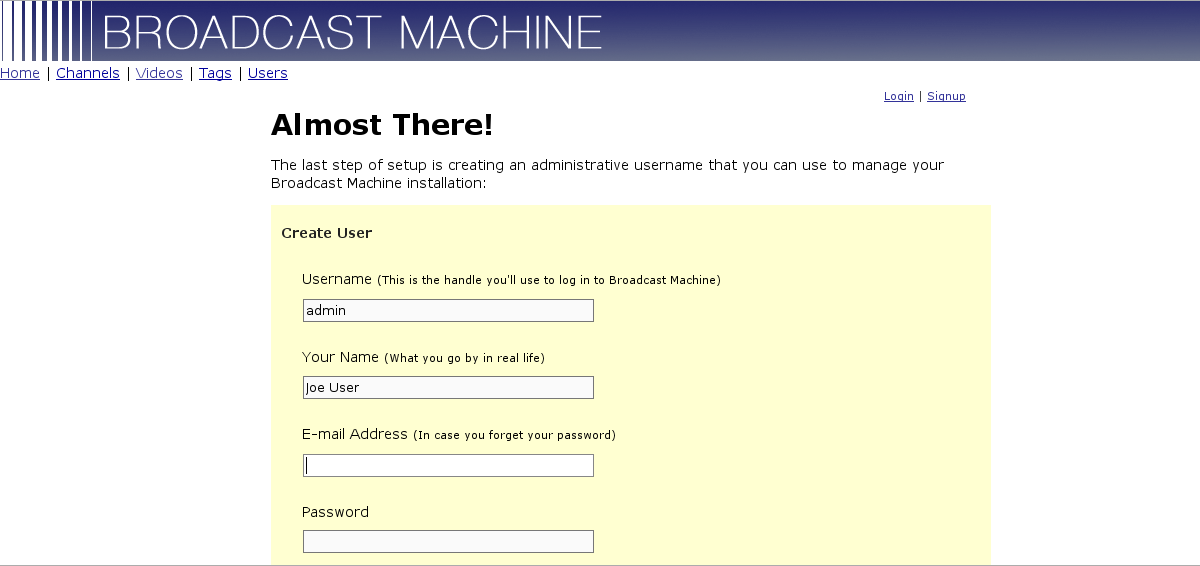
\includegraphics[width=150mm]{./images/setup3.png}
\caption{User Creation}
\end{center}
\end{figure}
On the third page, the user is prompted to enter in information for their first user. This is shown by Figure 5.3.
This user will be the \scare{superuser} and has the right to add other users or to escalate user permissions.

\subsection{Finished}
\begin{figure}[htp]
\begin{center}
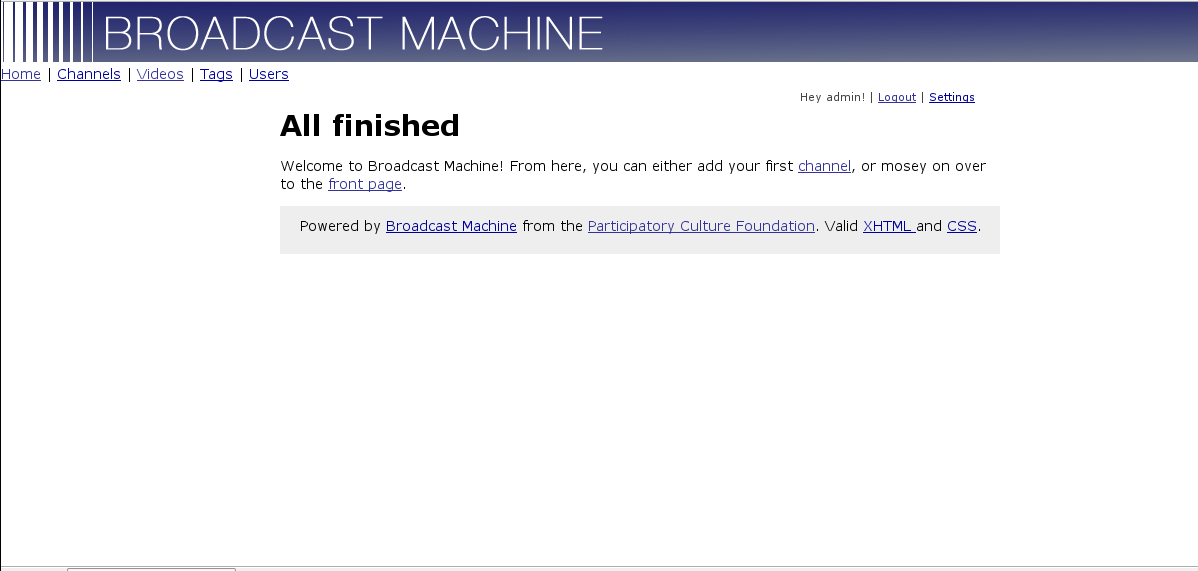
\includegraphics[width=150mm]{./images/setup4.png}
\caption{Finished Page}
\end{center}
\end{figure}

Figure 5.4 shows the fourth and final page is a simple confirmation that tells the user that they have successfully finished setting up the software.
From here, we provide prompts for the user to add a new channel or to take a look at their new front page.

\section{Channels}
The main component of Broadcast Machine are channels.
Channels offer a convenient way to group together videos.
Most people immediately understand the goal of a channel as a collection of thematically related content.
Our software provides an easy way for users to create, categorize and manage large amounts of video.

\subsection{All}
\begin{figure}[htp]
\begin{center}
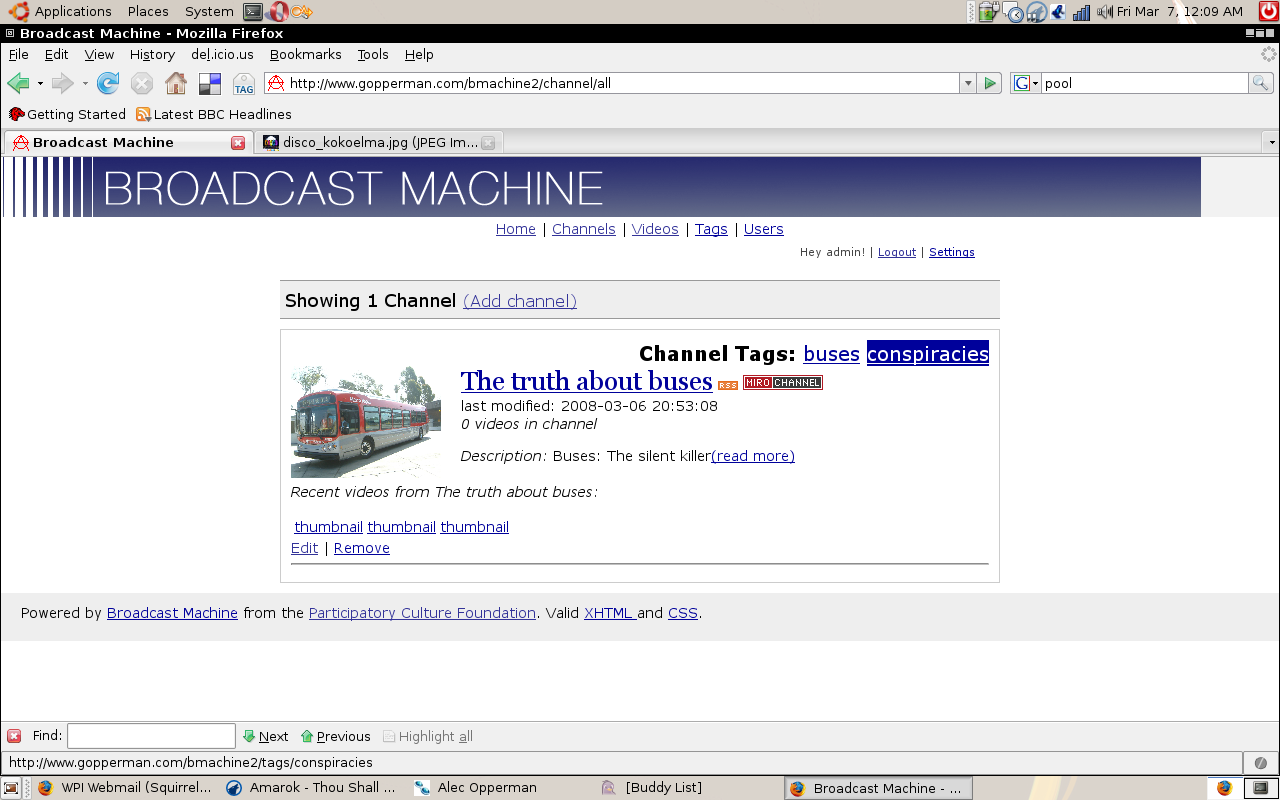
\includegraphics[width=150mm]{./images/channelall.png}
\end{center}
\caption{Viewing All Channels}
\end{figure}

Figure 5.5 shows the default display for the channels section, which is to show a few recent channels and a small sampling of videos from each channel.

\subsection{Show}
\begin{figure}[htp]
\begin{center}
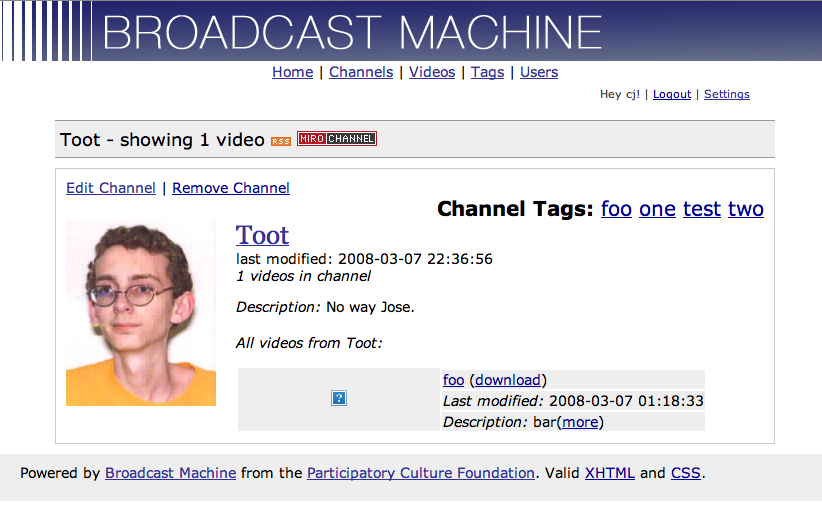
\includegraphics[width=150mm]{./images/channelshow.png}
\end{center}
\caption{Showing a Channel}
\end{figure}

Each channel can be viewed individually, as shown in Figure 5.6.
This allows the user to take a more in depth look at the channel.
In this view we display all of the information we have about the channel and then display a few of the recent videos.

\subsection{RSS}
\begin{figure}[htp]
\begin{center}
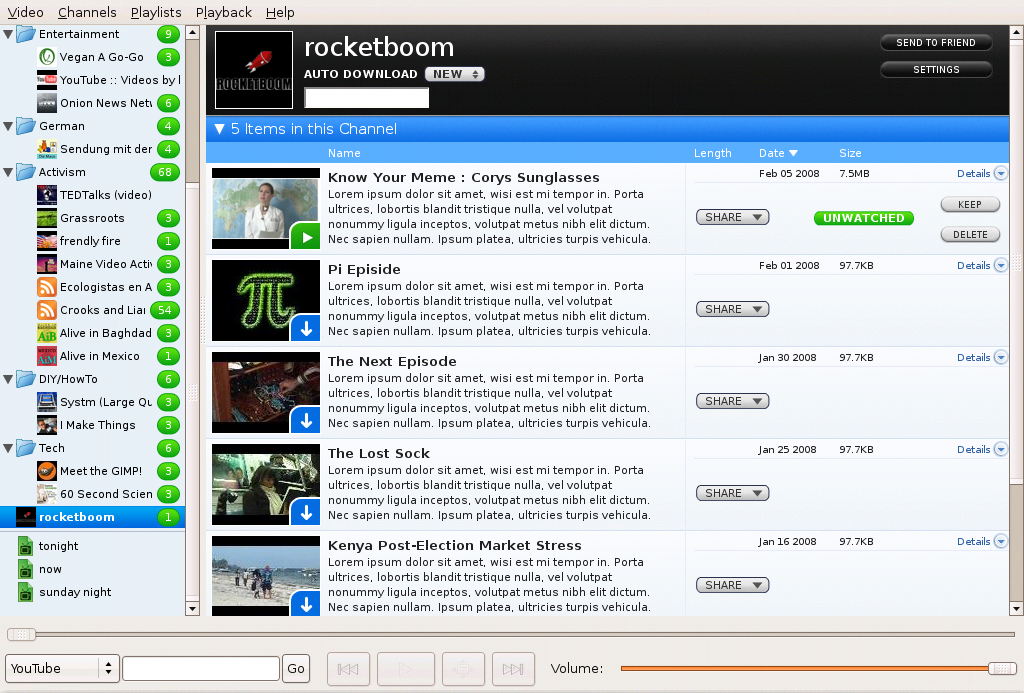
\includegraphics[width=150mm]{./images/channelrss.png}
\end{center}
\caption{Viewing a Channel's RSS Feed in Miro}
\end{figure}

All of the channels have an associated RSS feed.
The ten most recent videos that have been posted to the channel become a part of the RSS feed.
These feeds are important for integration with desktop clients such as Miro. Figure 5.7 shows the RSS feed for a given channel shown in Miro.
With this technology Broadcast Machine users can easily integrate their content with other services and clients.

\subsection{Add}
\begin{figure}[htp]
\begin{center}
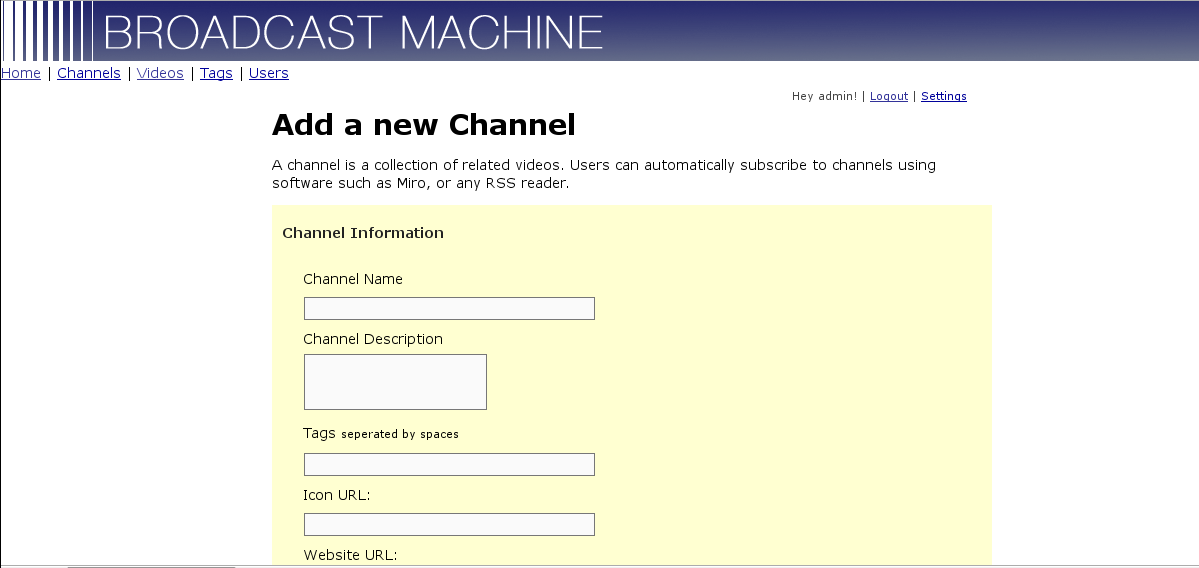
\includegraphics[width=150mm]{./images/channeladd.png}
\end{center}
\caption{Adding a Channel}
\end{figure}

None of this would be of much use if the software was lacking an interface through which to add channels. Figure 5.8 shows the interface for adding a video. With this dialog, an administrator can add a new channel and associate a few pieces of meta data.
We currently allow titles, descriptions, tags and icons to be attached to a channel.

\subsection{Edit}
\begin{figure}[htp]
\begin{center}
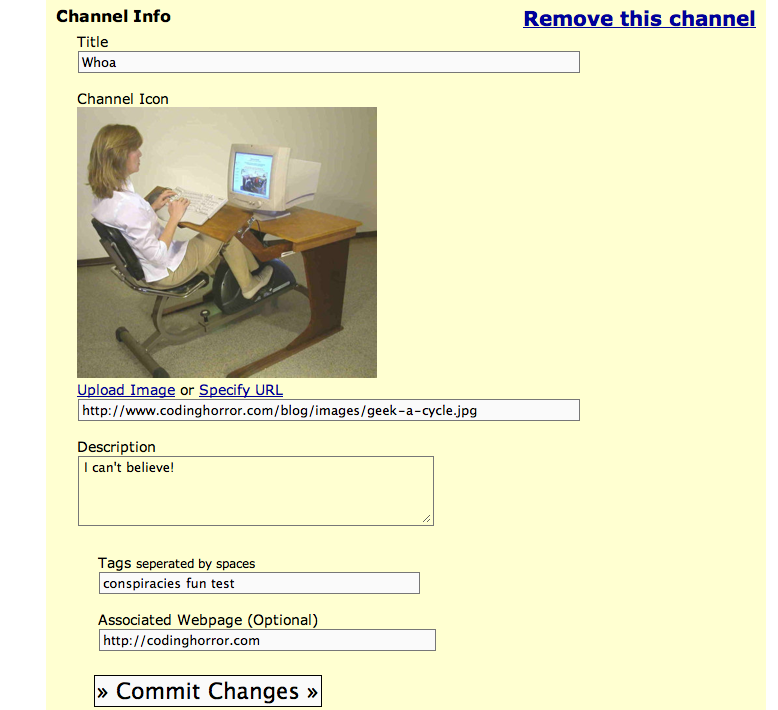
\includegraphics[width=150mm]{./images/channeledit.png}
\end{center}
\caption{Editing a Channel}
\end{figure}

The channel edit form (shown in Figure 5.9) is much like that of the add dialog, but this form comes pre-populated with the data from an existing channel.
Any piece of data that can be added can also be edited.

\subsection{Remove}
Nothing needs to be displayed for the remove action.
Instead, when an administrator goes to remove a channel, we simply alert them that their channel has been removed and then we forward them to the default channel page.

\section{Videos}
Videos are at the core of Broadcast Machine.
They are the most basic component of this application.
The video section of this software allows for all of the basic operations on a video.

\subsection{All}
\begin{figure}[htp]
\begin{center}
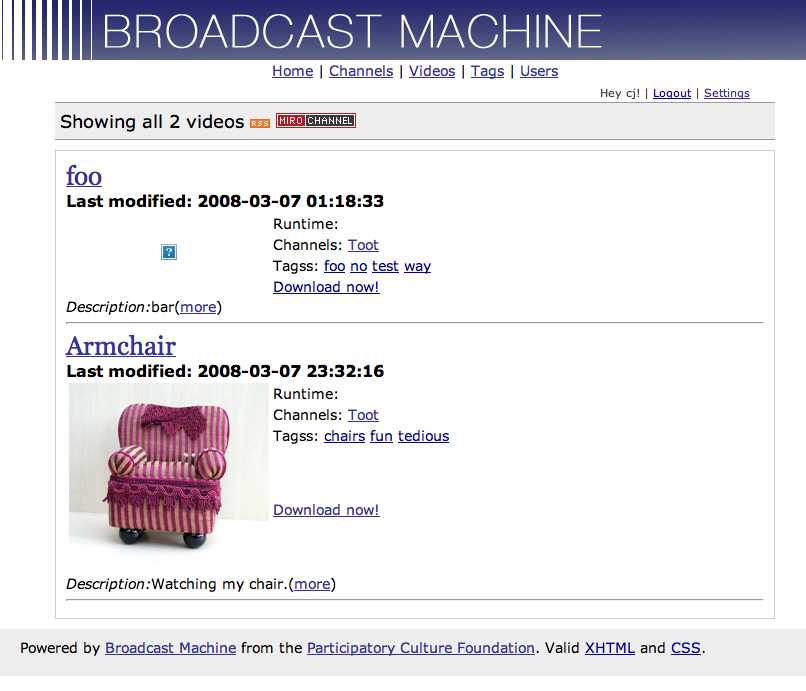
\includegraphics[width=150mm]{./images/videoall.png}
\end{center}
\caption{All Available Videos}
\end{figure}

Figure 5.10 shows the all videos view, which displays a number of the recent videos that have been added to the database.
This page serves as a good entry point into some of the videos that the user(s) have made available.

\subsection{Show}
\begin{figure}[htp]
\begin{center}
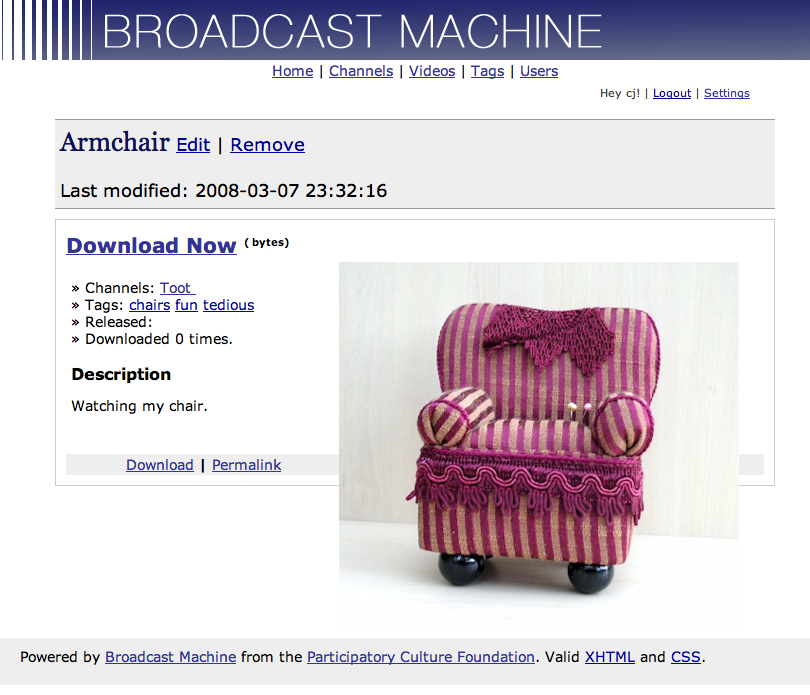
\includegraphics[width=150mm]{./images/videoshow.png}
\end{center}
\caption{Showing a Video}
\end{figure}

The show page, shown in Figure 5.11, displays a single video and all of the information associated with it.
This page gives the user a way to view meta data and to download the video itself.
It also serves as a jumping point to the channels that the video belongs to and to the tags that have been associated with the video.

\subsection{Download}
While the download portion of each video does not have a traditional HTML view, this is the most important part of the application.
This page redirects the user to a URI where the video file can be downloaded.

\subsection{Add}
\begin{figure}[htp]
\begin{center}
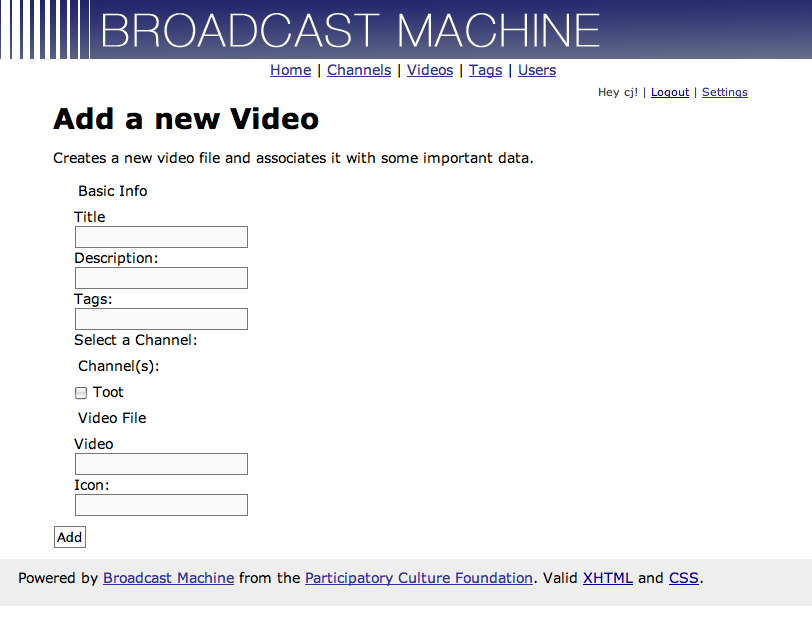
\includegraphics[width=150mm]{./images/videoadd.png}
\end{center}
\caption{Adding a Video}
\end{figure}

If a user is logged in and has sufficient privileges to add a video, they are presented with a form that allows them to fill in meta data. This is shown in Figure 5.12

\subsection{Edit}
\begin{figure}[htp]
\begin{center}
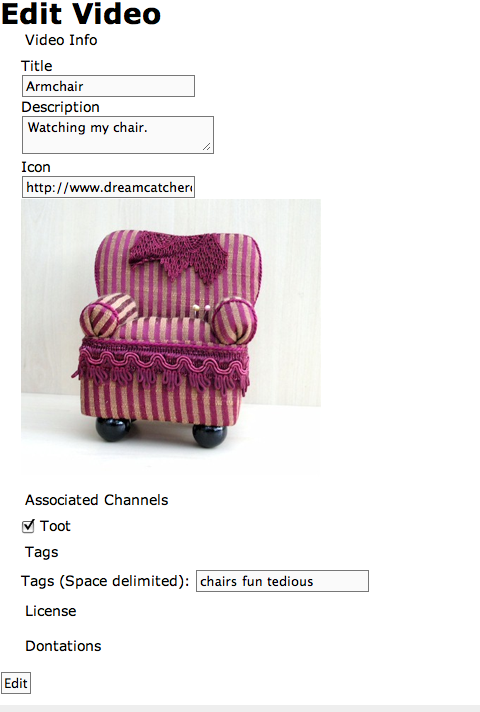
\includegraphics[width=150mm]{./images/videoedit.png}
\end{center}
\caption{Editing a Video}
\end{figure}

This view is much like the add view. It is visually similar except for it comes populated with data associated with the video. This view is shown in Figure 5.13.

\subsection{Remove}
There is no discrete XHTML view associated with the remove functionality, but an alert is passed onto the administrator who removes the video.

\section{Tags}
Tags are a convenient method for users to attach information to their videos.
Broadcast Machine offers the the ability to associate a group of single meaningful words to each video and channel.
These words allow the viewer to more easily pick through the content that is being presented.
Regardless of the channel or video, a viewer can immediately key in on some specific term and be able to retrieve a stream of content relevant to that term.

\subsection{All}
\begin{figure}[htp]
\begin{center}
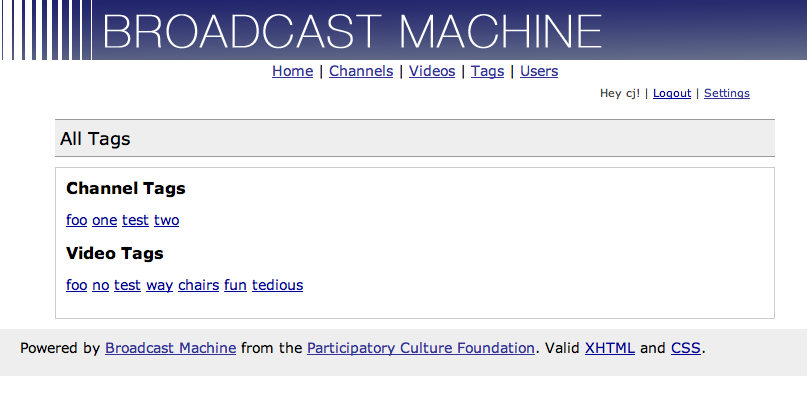
\includegraphics[width=150mm]{./images/tagall.png}
\end{center}
\caption{All of the Tags}
\end{figure}

As shown in Figure 5.14, this is raw tag output that allows users to see a bunch of the tags currently being used by channels and videos.

\subsection{Show}
\begin{figure}[htp]
\begin{center}
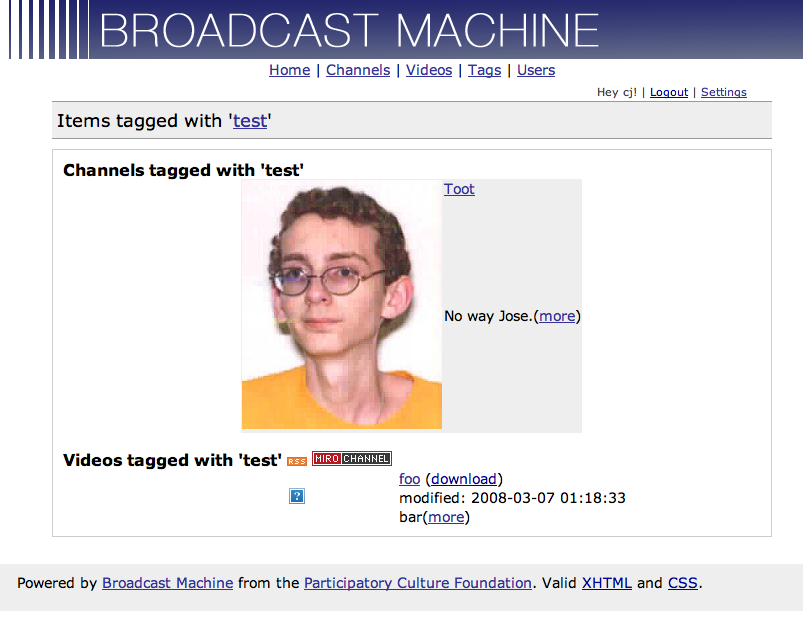
\includegraphics[width=150mm]{./images/tagshow.png}
\end{center}
\caption{Showing a Tag}
\end{figure}

As you can see in Figure 5.15, in this view there is a small sample of the channels and videos that have been associated with the given tag.

\subsection{RSS}
\begin{figure}[htp]
\begin{center}
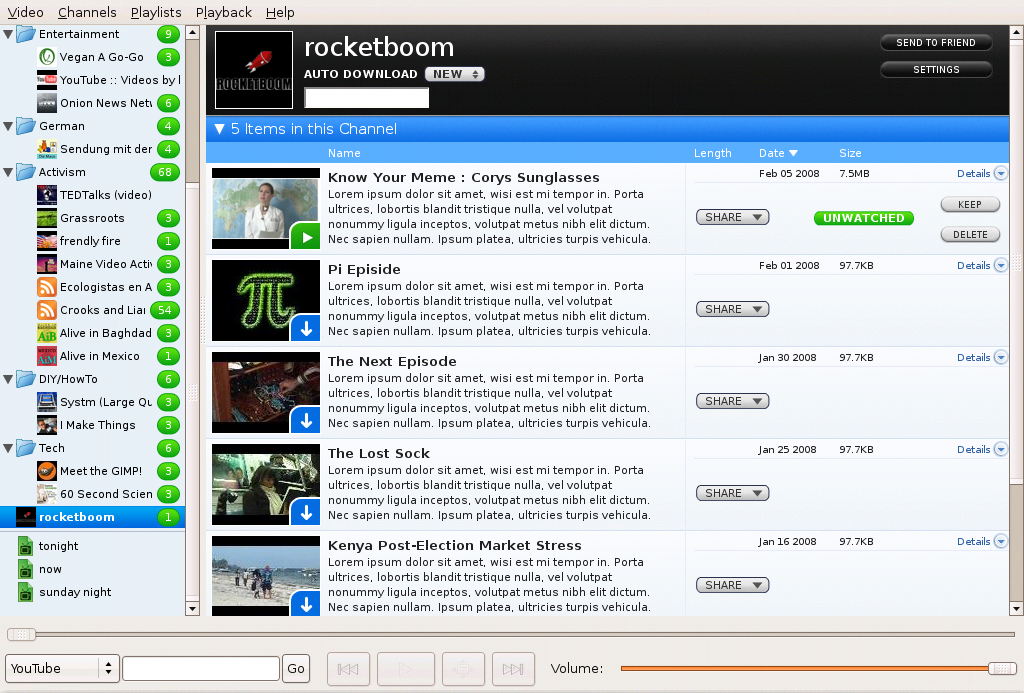
\includegraphics[width=150mm]{./images/channelrss.png}
\end{center}
\caption{Viewing an RSS feed}
\end{figure}
This view functions exactly like the previous channel RSS view that was discussed earlier.
Instead of keying in on channel data, this simply keys on tag data. See Figure 5.16.

\section{Users}
The users controller allows users and administrators to manage their and other's accounts.
This controller provides authentication mechanisms and a portal to certain amounts of user information.

\subsection{Signup}
\begin{figure}[htp]
\begin{center}
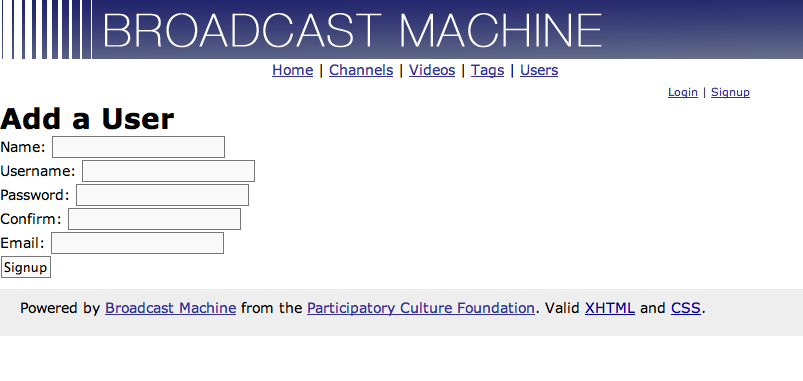
\includegraphics[width=150mm]{./images/usersignup.png}
\end{center}
\caption{Signing Up}
\end{figure}
As you can see in Figure 5.17, the super-user has control as to whether or not the signup pane is available to the public, but this dialog adds a simple way for users and administrators to add new accounts.
Each person is required to have a username and a password and we would prefer if they associated an email address and a name.

\subsection{Login}
\begin{figure}[htp]
\begin{center}
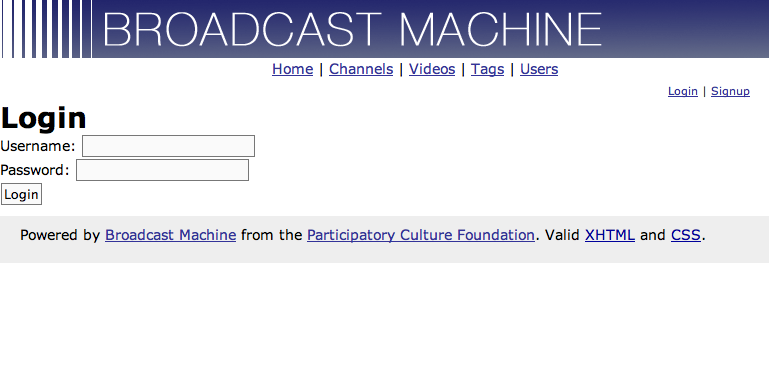
\includegraphics[width=150mm]{./images/userlogin.png}
\end{center}
\caption{Logging In}
\end{figure}
On the login page, as shown in Figure 5.18, the current user is prompted for their credentials.
Their username and password are requested and then authenticated.
If the credentials are correct, the user is marked as \scare{trusted}.
If not, then no mark is associated.

\subsection{Logout}
This is another piece of important functionality that is without an XHTML view.
The function is simple, it erases all of the session data currently set and alerts the user that they have logged out.
The user is then redirected to the home page.

\subsection{Show}
\begin{figure}[htp]
\begin{center}
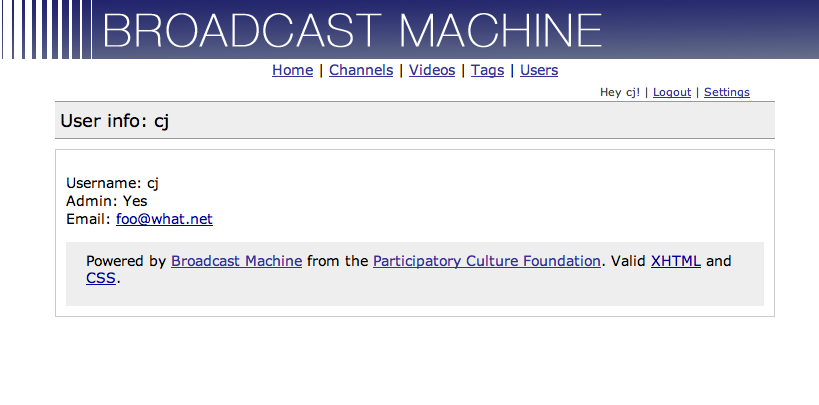
\includegraphics[width=150mm]{./images/usershow.png}
\end{center}
\caption{Showing a User}
\end{figure}
In Figure 5.19 you can see that at this point users are given the chance to view a single user and all of the data that is associated with that user.

\section{Summary}
In this chapter we showed how the software operates in a real-life situation. We showed the steps a user would take to install and 
configure their install of Broadcast Machine. 

\chapter{Results}

\section{Introduction}
Broadcast Machine has many components that work together to create a rich user experience. It is important to ensure that everything is 
working as expected, both in terms of functions as we--the developers--had planned and how typical users would expect the system to 
function.
Quality Assurance for Broadcast Machine was an ongoing process that began early on in our development cycles, in order to provide 
empirical benchmarks for code and layout correctness. 
An extensive system of unit tests were developed in order to rigorously test that all controller logic and model interactions in Broadcast Machine, while we later relied on user testing in order to verify that the presentation logic was also sound.

\section{Unit testing}
In order to ensure that Broadcast Machine's controller logic was (and is) consistently functional amongst dozens of revisions made by multiple developers, we developed a comprehensive set of unit tests that execute every controller function and verify that they return expected results. In order to perform these tasks, we implemented tests using SimpleTest, a PHP unit testing framework. SimpleTest uses basic assertions to prove that a given function behaves correctly, and then generates a simple report with the number of test case successes or failures.

\begin{figure}[htp]
\begin{center}
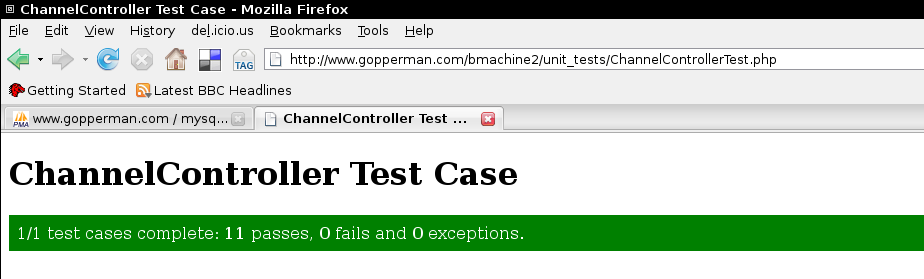
\includegraphics[scale=0.45]{./images/unittest.png}
\end{center}
\caption{ChannelController Unit Test}
\end{figure}

Unit tests for Broadcast Machine can be found in the unit\_tests folder, and may be executed simply by navigating to the test file in any web browser, as shown in Figure 6.1. While not entirely test-driven, our development process benefited greatly from good unit testing practices. Ensuring that all controllers passed their respective unit tests before checking in major portions of code helped prevent the introduction of bugs, as well as helped localize bugs to specific portions of code when they did occur. 

Although convenient for basic testing, Simpletest has several limitations that prevented us from testing all of our code through unit tests. Simpletest is unable to properly emulate persistent PHP sessions, which means that we had to test user authentication manually. However, since so many aspects of Broadcast Machine rely on authentication, we became confident that user-testing through our extensive use of Broadcast Machine throughout development was sufficient to ensure that the feature was working correctly. Similarly, unit tests are not able to make judgements about the correctness or aesthetic value of presentation logic. 

\section{Feedback}

In order to test Broadcast Machine's layout and usability, we relied on user testing and feedback. On February 23, 2008 we met with Mike Benedetti, the webmaster from Worcester's Community Cable Access (WCCA) Channel 
13. Mike is a part of the Internet video publishing community, as a member of Worcester Indymedia and as an independent journalist. Mike 
publishes the Snow Ghost Community Show\footnote{\url{http://www.wccatv.com/snowghost}} online for WCCA.
We introduced Mike to Broadcast Machine, and asked for some feedback on the user experience.
Our major goal was to determine if his expectations for the interface meshed well with the existing feel of the application.
Because of his experience with Internet video publishing, he was in a unique position to provide feedback on Broadcast Machine.

WCCA has recently begun putting all of their video content online, using Drupal with a number of modules as their content management system. 
Mike explained that there were a number of drawbacks with his current setup. 
Mike stressed that there was not yet a one-stop video content management system, although he did point out that there 
exist plugins and modules for existing CMS's that transforms them into a make-shift video CMS. 

We started our discussion by having Mike describe WCCA's video publishing process:

\begin{enumerate}
\item A content producer records a show in their studio. 
\item The show is edited and cut down to fit the time-slot.
\item The show is aired on the cable station. 
\item Mike uploads a high-quality copy of the video to archive.org. He must input various attributes of the video, including the title, text description, director, producer, production company, keywords and information about the audio and visuals. 
\item Archive.org's servers then convert the video into a number of file sizes and formats and make the files publicly available.
\item Mike embeds a lower-quality version of the file in a post using Drupal. Mike must re-enter all of the video attributes at this point.
\item The video is posted to the WCCA site and Drupal handles adding an entry to the video RSS file.
\end{enumerate}

After we talked with Mike about his setup, we opened up a browser and had him explore Broadcast Machine. At this point we 
asked him to follow links and describe what his exceptions for the pages were and compare his expectations to the 
content of our pages. 
It was valuable to hear that Mike's expectations for the views were somewhat different than what we had. 
There were a few specific UI suggestions that he had, but most important suggestion on how to visually present our data.
More broadly, Mike gave us a feel for where Broadcast Machine fits into the landscape of Internet video publishing. 

He seemed to be hopeful about our project and it might be a good fit for his needs.

Mike explained that it made more sense to him to have the videos appear in a more traditional blog layout, with clear 
differentiation between posts, and with a publish date clearly indicated. 
He also pointed out that we needed to make it clear that the RSS feeds were video feeds that could be used with 
programs like Miro. To bring attention to this feature, we moved icons for RSS and Miro subscription links to be more prominent on pages where feeds are available, and also updated several templates to clearly differentiate between video posts with better-presented information. Mike indicated that he was confused about what data was in the RSS feeds, based on their placement. We discovered that it needed to be made more clear that the video feeds had enclosures, and moved the RSS icons to a location on the page that more clearly indicated their content. In accordance with Mike's suggestions, we also edited templates for consistency in ordering videos and channels.

As was mentioned earlier, WCCA uses archive.org as their long-term storage. 
Mike suggested that Broadcast Machine would be a more appealing piece of software if, in a future release, it 
incorporated an easy mechanism for external storage solutions. 
We looked at WCCA's account and found that there is an XML API provided for archive.org to integrate with external 
software. The XML API would make the implementation of a function to scrape data from archive.org an easy task for future releases of Broadcast Machine. Having Broadcast Machine automatically grab data from archive.org would streamline WCCA's process for uploading files. Mike also suggested integration with several other storage providers, including Amazon's S3 service. While certainly a good idea for the future, implementing robust integration with several different services is a major task, and was outside the scope of this project's time constraints.

Mike recalled that the previous version of Broadcast Machine was based on BlogTorrent, an implementation of the BitTorrent transfer protocol for blogs. 
However, he also noted that he was unable to get BitTorrent support to work with previous installs of Broadcast Machine, an experience that several other users of the earlier BM often shared. 
Mike suggested we add some sort of BitTorrent integration.
While the current Broadcast Machine does allow users to upload or link to .torrent files and share them, we identified the need for an integrated BitTorrent server in order to automatically seed, or upload videos. We had previously considered adding this feature. However, we found that most hosting providers do not allow server-side sharing of torrents in any regard. Due to this constraint, we decided to abandon implementation of this feature, but are now reconsidering it for advanced users running their own web servers.

Meeting with Mike Benedetti gave us a good perspective on how video publishers would react to Broadcast Machine. 
We did not incorporate all of his suggestions, but we did make a number of changes based on his ideas. 
It was encouraging to hear that Broadcast Machine could grow to fill a vital niche in the video publishing field, and might even be utilized by WCCA in the future.

\chapter{Future Work}
While this project has done much work to make Broadcast Machine a piece of modern video management software, there are many features that should be implemented in order to provide the best user experience possible.
Fortunately, Broadcast Machine will live on longer than this current project.
Our group hopes to continue to cultivate this application as an open-source project after this MQP.
Opening this code-base to a community and encouraging all types of hobbyists to contribute will allow us to implement a few of the features that we think would be beneficial to the software.

One of the first features that this project did not implement was BitTorrent support.
The initial version of Broadcast Machine was hailed as being one of easiest ways to distribute content via this de-centralized network, but few people were able to take advantage of this, due to numerous bugs.
We think that this feature is still important to goals that Broadcast Machine tries to accomplish.
The ability to save bandwidth and provide free redundancy is immensely important.
These features should be relatively easy to implement as most of the code for these features is available in the initial version of the software.

With the rise of online video, many content providers have decided to make their video viewable online through the use of a Flash applet.
The use of this embeddable program allows the provider to make video viewable on almost any computer on any platform.
If the user has encoded their video using the FLV codec or the H.264 codec, a well-designed SWF can provide the playback interface.
While this interface can only be provided through the use of a closed-source application framework, it is perhaps the most usable method for providing a video player.
Fortunately, with the use of file-type detection and the adaptation of open-source Flash applications we feel that this feature would be important to provide.

The next feature that would be most beneficial to the user-base would be robust internationalization support.
The computer world largely deals with English as the default language in which to implement software, the majority of the world does not function in English.
There are a large number of users who would benefit through the existence of a multi-language framework.
The ability for Broadcast Machine to be translated into multiple languages would be a tremendous boon to users across the world and would increase the number of people that our package would be immediately usable to.
This feature would be relatively easy to implement as well.
Because of the architectural decisions that we have made, the translation would only take a few hours to a native speaker of any language.
Given that we are able to find people willing to volunteer for this job, this feature would be of great benefit.

The last feature that our team thought useful was AJAX support.
AJAX has become popular for use in web applications lately as it allows for asynchronous functions that are often found in desktop applications.
Through the use of these methods we would be able to allow administrators to edit the content on their pages without having to refresh the page.
All of the necessary information changes hands in the background.
This feature would be a bit harder to implement.
Many changes would be needed to properly interpret the new flow of information, and integrating these client-side programs would likely take a long time.
The benefit would be increased ease of use; Broadcast Machine would \scare{feel} much like a desktop application.

All of these features are certainly within reach.
The benefits to the users afforded by their implementation versus the effort required is certainly reasonable.
Hopefully Broadcast Machine sees these features added to its code base in the coming months.
Its life as an open source project and the addition of other contributors should speed the addition of these features that we have not had time to add.
 
\chapter{Conclusion}
Internet video is one of the fastest growing information mediums in society today. Advances in communications technology has allowed video publishers to share their work with thousands across the world. Several centralized hosting services currently exist for hosting videos, but none give publishers full control over how their work is presented and distributed. Broadcast Machine, an abandoned open-source project by the Participatory Culture Foundation, attempted to fill this niche, but ultimately failed due to instability.

By examining the architecture and downfalls of the previous Broadcast Machine, we were able to thoughtfully design a stable successor that 
enables video producers to easily publish their work on the Internet. We have created a robust architecture that is easy to use for publishers, viewers, designers, and developers alike. The new Broadcast Machine allows publishers to share high quality video on their own terms, and without special technical knowledge.

We hope that this new version of Broadcast Machine enjoys the same amount of popularity as its predecessor.
Our team feels that this software can be a useful tool and has the possibility to change the current environment for Internet video.
As an open source project, we hope our continued dedication will attract additional developers so that this software may progress long after this project is over.

\appendix
\chapter{Former Broadcast Machine Documentation}

\section{Data Model}


\subsection{Instances}
The instance table was used to prevent two versions of Broadcast Machine from using the same database. In the previous version of Broadcast Machine, if more than one site was using the same database, a warning was displayed on the main page of the administrative interface. The table consists of a hash string of the hostname (id), and a timestamp for when the instance was created (time). 


\subsection{Stats}
The stats table allowed the user to keep track of the number of user downloads for each video. It contained a unique hash of the filename (id), and an integer for the number of downloads (downloads). The table has a one-to-one relationship with files.


\subsection{Channels}
The channels table was used to store metadata about specific RSS video feeds, or channels. This data was used to generate the channel view and RSS feeds for each channel, which is how most users interact with the application. 
%Show a screenshot of the channel view, perhaps?
It contained a unique integer identifier (ID, the primary key), A text explanation of the channel (description), and integer number for when the channel was made (Created), a text title for the channel (name), fields for URLs of linked icons, libraries, and the channel's main website (Icon, LibraryURL, and WebURL, respectively), a field to designate the publisher (Publisher). In addition to this, it has several tiny int values that served as settings flags, with 0 being false, and the default value, and 1 being true. This includes OpenPublish, RequireLogin, and NotPublic. OpenPublish allowed administrators to designate whether or not non-administrative users were allowed to publish videos to a channel. RequireLogin was used to determine whether or not users must be logged in to view the channel. If NotPublic was set, the channel itself would be hidden from anonymous users.
It also contained CSSURL, which would store a link to an external style sheet to be used in rendering the channel page.


The channel\_options table keeps track of the individual settings for a given channel. Each record in the table contains an integer reference to the channel it refers to (ID). Several boolean flags determined which information about a video would be shown on the channel view: Creator, Description, Filesize, Keywords, Length, Published, Thumbnail, Title, Torrent, URL. There is also a tiny int field called SubscribeOptions, whose default value is 7. This value determines which subscription links will be made available to users (RSS, Democracy, and iTunes, which requires direct URLs to be enabled in the site settings). In this field, RSS is represented by a value of 1, Democracy by a value of 2, and iTunes by a value of 4. Adding together the values of available subscription links determines the field's value. For example, A value of 7 means that all links are available for use, while a value of 1 would mean that only RSS could be used. A value of 6 would mean that iTunes and Democracy subscription links should be made available. 


The channel\_files table records associations between the channels table and the files table (see below). In other words, it allows Broadcast Machine to keep track of which files belong to which channel, which is essential to the channel view and RSS feeds. It contains a reference to the channel in question (channel\_id), the hash of the file (hash), and integer timestamp (thetime). The primary key is channel\_id and hash, meaning that there can't be more than one record for any channel and file pair.


The channel\_sections table allows channels to be split up into several subsections. From experience, this seems to be widely unused by BM's user base, and is also not implemented in the RSS view. As such, it may be deprecated. The table itself contains an integer reference to the channel the record refers to (channel\_id) and the name of the section (Name). The table also shares a one-to-one relationship with the channels table.


Like channel\_files, the section\_files table tracks which files are associated with which sections. The table contains a reference to channel\_id, a reference to the name of the section, and the hash of the file. The combination of those three fields are a primary key and must be unique.


\subsection{Videos}
The table for storing video information is the files table. This information is used to render the details page for each individual video. The files table contains a unique integer identifier for each video (ID), an ineger for when the file was created (Created), the name of the file (FileName), the name of the person who created the channel (Creator), a text summary of the file (Description), a title (Title), an optional link to a transcript for the hearing-disabled (transcript), a link to a website for more information(Webpage), an optional donation code (donation\_id), boolean flags for Excerpt, Explicit, ignore\_mimetype, and External properties, and URL, in case the file was linked to externally. It also contains a link to an image thumnail of the video (Image), name and URL of the license used to distribute the video (LicenseName, LicenseURL), the MIME-type of the file (Mimetype), an integer for the date published (Publishdate), and the date of the video release via three fields: ReleaseDay, ReleaseMonth, and ReleaseYear (all are integers). Also included is a short string called Rights, which is slightly redundant due to the License field. 


Records of people who have contributed to the making of a video were stored in the file\_people table. This allowed administrators to include conprehensive credits for anyone working on the video. The table contained an identifier for which video the credit refers to (ID), their name (name), and what they were credited for (role). The combination of these three values were required to be unique as a primary key.


\"Tags\", or categories to classify videos by, were stored in the file\_keywords table. This allowed administrators to classify videos by category, so that users could browse videos in that category across many channels. This table contained an ID reference to the video, and then the keyword that the video would be tagged by. Although one video may have had many tags, no video could have two identical tags.


\subsection{Donations}
The donation table stores information on how users can contribute to the makers of a video. This allowed the generation of donation links to be displayed alongside a video in the video view, as well as from within Democracy and the RSS feed for the channel. Users could use these links to contribute to the makers of the video. Each donation record had a unique ID, an e-mail address (email), a short description (title), and a longer text donation pitch (text). Putting this information in its own table allowed publishers to frequently associate videos with the same donation info, as this info rarely changed. 


The donation\_files table links together donation info with video info. The table conatined the id of the donation info, as well as the hash id of the video (hash). Each video could only be linked to one set of donation information, so id and hash are both primary keys.


\subsection{Users}
The user table contained information about registered users. This table contained an alias for each user (Username), the user's real name (Name), their encrypted password (Hash), their e-mail address (Email), when they registered (Created), and their permissions information (IsAdmin, IsPending). 


The newusers table tracked only those users who have not verified their account. This allowed functionality to prevent scripted bots to spam Broadcast Machine installations with open registration, by requiring that all users verify their e-mail address. The table included a filehash, their password (Hash), their e- mail address (email), IsAdmin, and when they created the account (Created).


\subsection{Settings}
Settings for the website itself was stored in a B-Encoded flat file. This allowed users to customize site security features, as well as which features they wanted to use. This is also where essential information such as database connection settings were stored. These fields include whether or not new user registration was allowed (AllowRegistration), whether or not they required approval (RequireRegApproval), whether or not they needed to verify their account (RequireRegAuth), whether or not users could upload or download anonymously (UploadRegRequired and DownloadRegRequired, respectively), the default channel (DefaultChannel), whether the site has channels that anyone could modify (HasOpenChannels), their current site layout (theme), title of the site, the site description, an image associated with the site, the base url for the site (baseurl), database connection settings (mysql\_prefix, mysql\_host, mysql\_username, mysql\_password, mysql\_database, and mysql\_verified), and BitTorrent sharing settings (Ping, sharing\_enable, sharing\_auto, sharing\_python, sharing\_actual\_python, minport, maxport).

\end{document}

